%                                                                 aa.dem
% AA vers. 9.1, LaTeX class for Astronomy & Astrophysics
% demonstration file
%                                                       (c) EDP Sciences
%-----------------------------------------------------------------------
%
%\documentclass[referee]{aa} % for a referee version
%\documentclass[onecolumn]{aa} % for a paper on 1 column  
%\documentclass[longauth]{aa} % for the long lists of affiliations 
%\documentclass[letter]{aa} % for the letters 
%\documentclass[bibyear]{aa} % if the references are not structured 
%                              according to the author-year natbib style

%
\documentclass{aa}  

%
\usepackage{graphicx}
%%%%%%%%%%%%%%%%%%%%%%%%%%%%%%%%%%%%%%%%
\usepackage{txfonts}
%%%%%%%%%%%%%%%%%%%%%%%%%%%%%%%%%%%%%%%%
%\usepackage[options]{hyperref}
% To add links in your PDF file, use the package "hyperref"
% with options according to your LaTeX or PDFLaTeX drivers.
%
\begin{document} 


   \title{The variability  of Betelgeuse explained by surface convection}


    \author{{ Q.~Pilate}\inst{1},{ A.~L{\'o}pez Ariste}\inst{1},{ A.~Lavail}\inst{1},{ Ph. Mathias}\inst{1} }

   \institute{IRAP, Universit\'e de Toulouse, CNRS, CNES, UPS.  14, Av. E. Belin. 31400 Toulouse, France 
             }

   \date{Received ...; accepted ...}

% \abstract{}{}{}{}{} 
% 5 {} token are mandatory
 
  \abstract


   \keywords{
               }

   \maketitle
%
%-------------------------------------------------------------------

\section{Introduction}

Betelgeuse is a prototypical red supergiant (RSG) known to be a semi-regular variable. Several periods can be found in the 
literature usually clustered around the so-called long secondary period (LSP) of 2000 days and other more or less well defined 
periods around 400 and 200 days. Such periods are often linked to radial pulsation modes,   and have been used to model 
the characteristics of the resonant cavity, hence the size of the star and eventually its evolutionary stage \cite{XXX}.


At the end of 2019, Betelgeuse reached a historical minimum in its luminosity, called the great dimming \citep{guinan_fall_2020}. 
From interferometric data, we know that this event was caused by a cloud of dust close to the line of sight \citep{montarges_dusty_2021}. 
Interferometric images show a huge drop in luminosity in the southern hemisphere of Betelgeuse, leading to this dimming. In this event it was clear that a change in brightness was not due to any kind of pulsation but to a change on the 
brightness distribution over the stellar disk due to the presence of large quantities of dust. While this may be seen as 
a singular event, it brings up the question whether all changes in brightness cannot be due to similar changes in the brightness 
distribution over the disk, unrelated to any pulsation phenomenon. 




Betelgeuse is known to present large convective cells with life times in the order of one to two years and measurable changes 
in the span of one week. Bright convection cells near disk center will increase the integrated brightness of the star when 
compared with other situations where such cells are found near the edges. So even without calling for the formation of 
dust or other changes in opacity, one may argue that the simple evolution of convective patterns of the star may create a variability. Such 
variability could be expected to be random, but will present quasi-periodicities related to the typical time scales of the 
convective patterns. 

Since the end of the Great Dimming event, Betelgeuse has continue its random variation of brightness. 
Interestingly, 
it has been shown by \cite{jadlovsky_analysis_2023} and \cite{dupree_great_2022} that the periodicity of Betelgeuse has changed after the dimming. Using the light curves from AAVSO, 
the authors showed that before the dimming, the dominant period of Betelgeuse was around 400 days. However, after the dimming, this period has changed and 
is now shorter, around 200 days. It means that, after the dimming, there was a change in the behaviour of the atmosphere of Betelgeuse: the period is now
shorter than before the dimming. Our analysis is based on this change of periodicity. 
Faced with the dramatic change in stellar parameters and age that such change in a pulsation period would 
require, our interest in an alternative explanation of the variability
in terms  of convective patterns arose. In order to address this question we shall seek for such typical periods of 1000, 400 and 200 days in  
observational proxies related to the convective activite but unrelated to pulsations and which cannot be directly linked to brightness?

Linear polarization in the atomic lines of the spectra of Betelgeuse, discovered by \cite{auriere_discovery_2016}, has been interpreted as the joint action of 
two mechanisms. First the depolarization of the continuum by atoms which absorb linearly polarized light and re-emit unpolarized light, the 
continuum photons being polarized by Rayleigh scattering. This depolarization produces signals with an azimuth symmetry over the disk that 
would  cancel out the net linear polarization on a homogeneous disk. Thus it must be combined with an inhomogenous disk to produce the net linear polarization 
signal observed. This interpretation suggested the possibility of mapping those brightness inhomogeneities. This has been done by \cite{lopez_ariste_convective_2018} 
even producing 3-dimensional images of the atmosphere of Betelgeuse \citep{lopez_ariste_three-dimensional_2022} when taking advantage of the different height of formation of 
different lines in the spectrum of Betelgeuse. The images produced compare very well with cotemporaneous images made with interferometric 
techniques and show clear convective patterns, akin to solar granulation.

Linear polarization observed in the atomic lines is therefore a proxy of convection, unrelated to radial 
pulsations but linked to the brightness inhomogeneities due to the convective patterns in Betelgeuse. If one can find the aforementioned periods 
in linear polarization, we must conclude that these periods are related to the convective activity which originates those linear polarization signals
and unrelated to any radial pulsation phenomena. This is the purpose of the present work.



\section{Searching for periodicities in the polarization spectra of Betelgeuse}

Betelgeuse has been observed for the last 13 years with Narval and Neo-Narval at the Telescope Bernard Lyot. These two instruments measure the polarization 
over the visible spectra of Betelgeuese (390-1000 nm) with high spectral resolution (R=65000) and high polarimetric sensitivity. Despite 
this high sensitivity, the signal-to-noise ratios are not sufficient to measure the weak polarization signals in individual atomic lines of the 
spectrum. These amplitudes are today known to be of the order of $10^{-4}$ times the continuum intensity, and only excepcionnaly do they 
reach amplitudes of $10^{-3}$ the continuum. In these exceptional observations, enough photons can be accumulated per spectral bin to 
see the linear polarization signal above noise \citep{auriere_discovery_2016}. Most commonly, the amplitudes of linear polarization are below noise levels. In those 
occassions we have to add up the signals of thousands of lines to reduce the noise and increase the signal-to-noise ratios. This line addition 
is done through a technique called Least-Squares Deconvolution (LSD) \citep{donati_spectropolarimetric_1997} and assumes that the 
linear polarization signal is similar 
in all spectral lines up to scale factors in the sampling and amplitude. This technique has been successfully used in the past to measure 
magnetic field distributions over stellar surfaces and it is now used to produce images of the brightness distributions in the photosphere 
of Betelgeuse and other red supergiants as cited in the Introduction. 

In this work we shall look into the signals produced through these line-addition techniques, and which produce a pseudo-spectral line in intensity 
and linear polarization which does not belong to any atomic species in particular but to an average of all of them present and emitting in the 
photosphere of Betelgeuse. After such procedures of line addition, these signals carry the coherent signals present in the photospheric lines, but the particularities of this or 
that spectral line are erased. All these data has been presented before by \cite{auriere_discovery_2016}, \cite{mathias_evolution_2018} and 
\cite{lopez_ariste_three-dimensional_2022}, which also give details on observing times and conditions as well as more detailed description 
on the data reduction \footnote[1]{Beyond a 2-year proprietary embargo, and up to technical issues, all these data is available through 
PolarBase (http://polarbase.irap.omp.eu/).}



%\subsection{Lomb-Scargle periodograms of the profiles}

Trying to find periods in an astrophysical context carries the hurdle of unevenly spaced observed data. To overcome this issue, 
we used the Lomb-Scargle (hereafter LS) periodogram \citep{lomb_least-squares_1976,scargle_studies_1982}. For a given set of data, it fits sinusoid functions 
using least-squares at each frequency between the first and the last observation. The better the fit, the higher the power attributed to the frequency. 
We apply this technique to the  LSD profiles of Stokes I, U and Q of Betelgeuse observed at the TBL during 
that span of 13 years. 


We first computed the LS periodogram at each wavelength of the LSD profile, between -25 km/s and 80 km/s to span the entire 
signal present in the LSD profile. \cite{lopez_ariste_convective_2018} found the most blueshifted signal towards -20 km/s, 
and interpreted it as  the maximum velocity of the rising plasma, seen from the Earth. The most redshifted signal was found at 40 km/s. 
This velocity is interpreted
as the rest velocity of the star in our reference frame. Seldom, signals at velocities larger than 40 km/s can be found 
and can be interpreted as either dark and cold plasma falling back to Betelgeuse, 
or to rising plumes of plasma located in the hidden face of Betelgeuse,
and rising so high that they appear above the limb.





% The LS periodogram  computed for each frequency 
% in the LSD profile must show periodicities around the LSP, but also on the 400 days and 200 days period. If the LS periodogram finds a periodicity at a
% given wavelength, it would appear as a strong LS power. However, we expect a change in the periodicity after the dimming. 
% This would lead to a decrease in the Lomb-Scargle power. By comparing LS periodogram before and after the dimming, we expect to see a change in the LS power,
% especially at the 400 days period. 

Figures \ref{LS intensity},\ref{LS Q},\ref{LS U} and \ref{LS linear polarization} show the Lomb-Scargle periodogram in normalised power of the LSD profile of respectively 
the intensity, stokes Q, stokes U and the linear polarization. 
%The abscissa is the frequency (in $\mathrm{days^{-1}}$), while the ordinate is the heliocentric radial velocity in km/s. 
For each figure, the upper panel is the LS periodogram with data taken before the great dimming of Betelgeuse, that is from 2013 to the beginning of 2019. 
The lower panel is the LS periodogram for the whole period before and after the dimming: from 2013 to 2023. The white dashed lines mark the different 
periods found in the literature: the LSP at 2000 days, the fundamental pressure mode at 400 days and its first overtone at 200 days.  

\begin{figure}[!h]
    \centering
    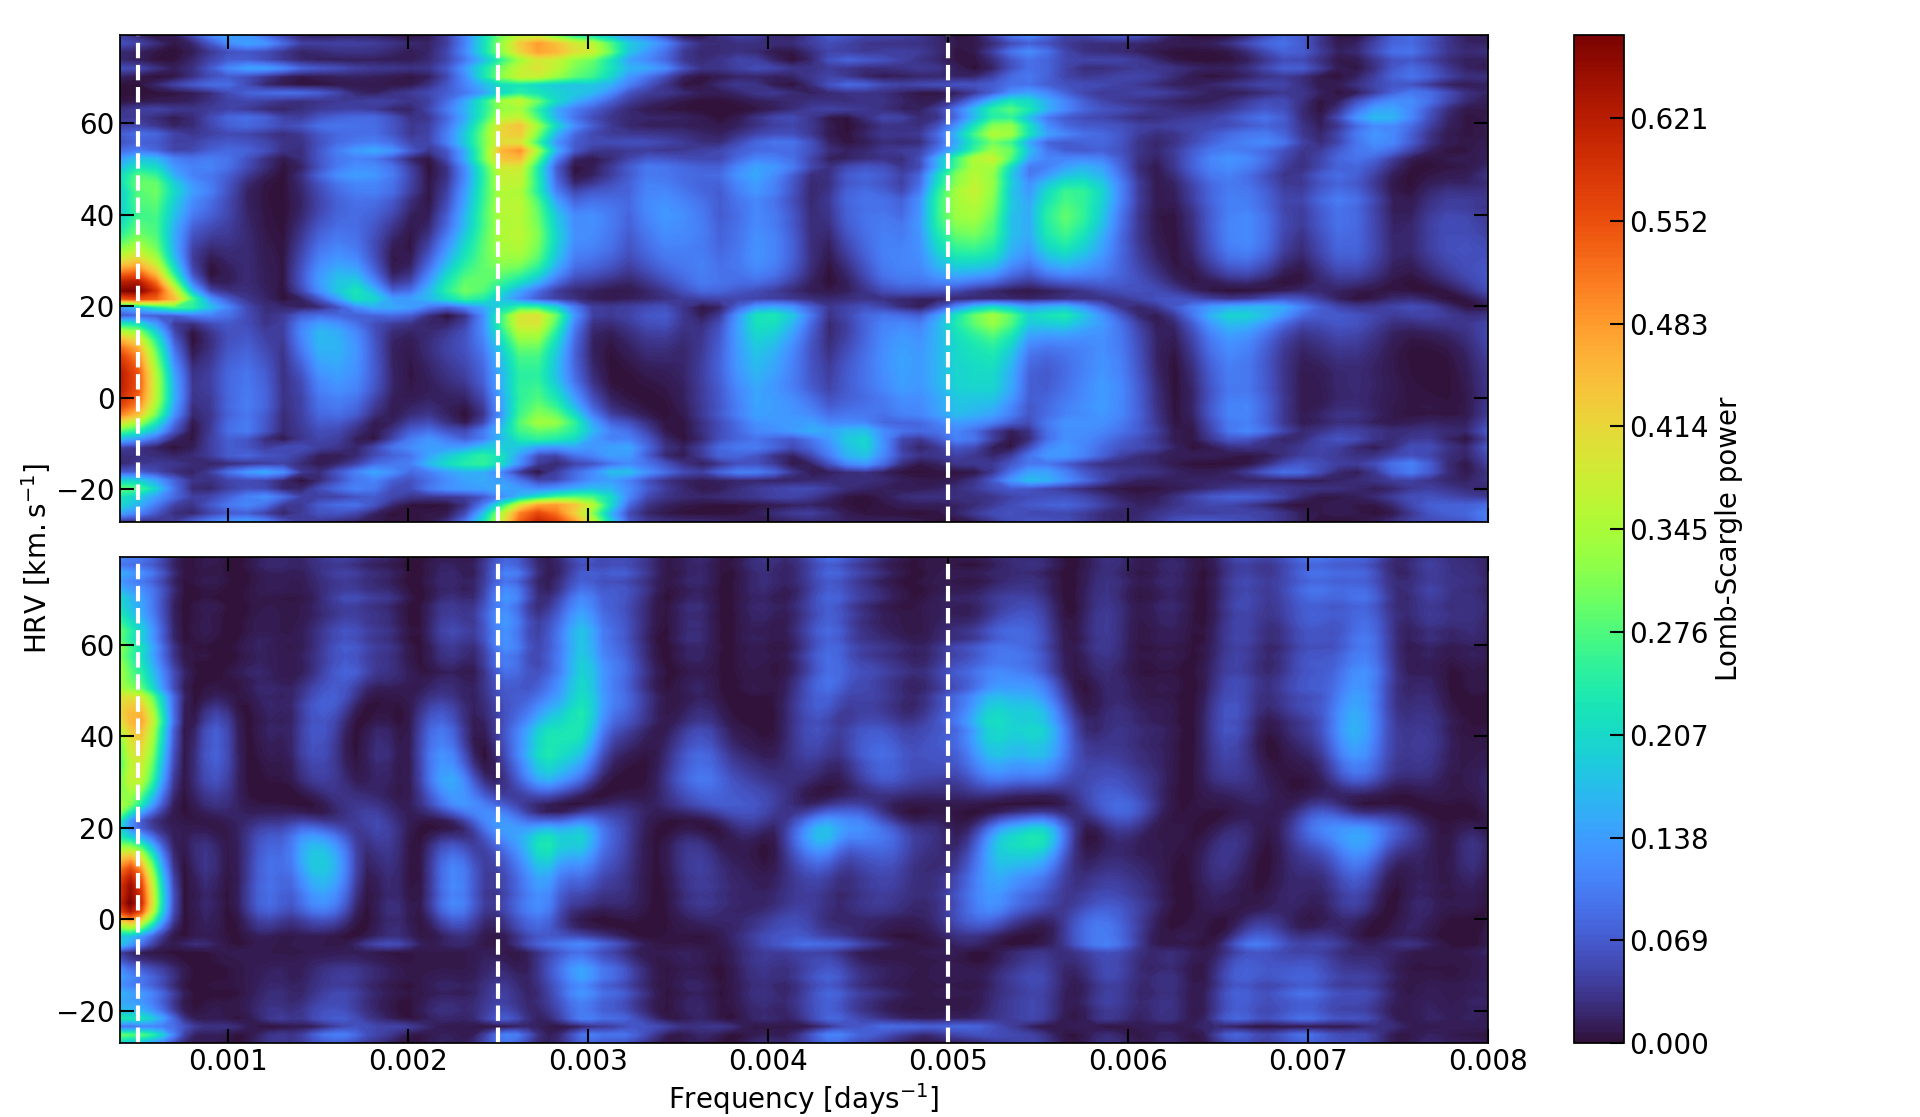
\includegraphics[width=0.5\textwidth]{Lomb-Scargle Intensity.png}
    \caption{Lomb-Scargle periodogram of the LSD profile of intensity. 
    The upper pannel is the LS periodogram for data before the great dimming while the lower panel is the periodogram from the all dataset.
    The ordinate refers to the velocity in the heliocentric radial velocity in km/s. The abscissa is the period in $\mathrm{days^{-1}}$. 
    The three white dashed lines represent respectively (from left to right) the LSP at 2000 days, the 400 days period and its first overtone at 200 days. 
    The Lomb-Scargle power refers to the quality of the fit from the LS periodogram. }
    \label{LS intensity}
\end{figure}

\begin{figure}[!h]
    \centering
    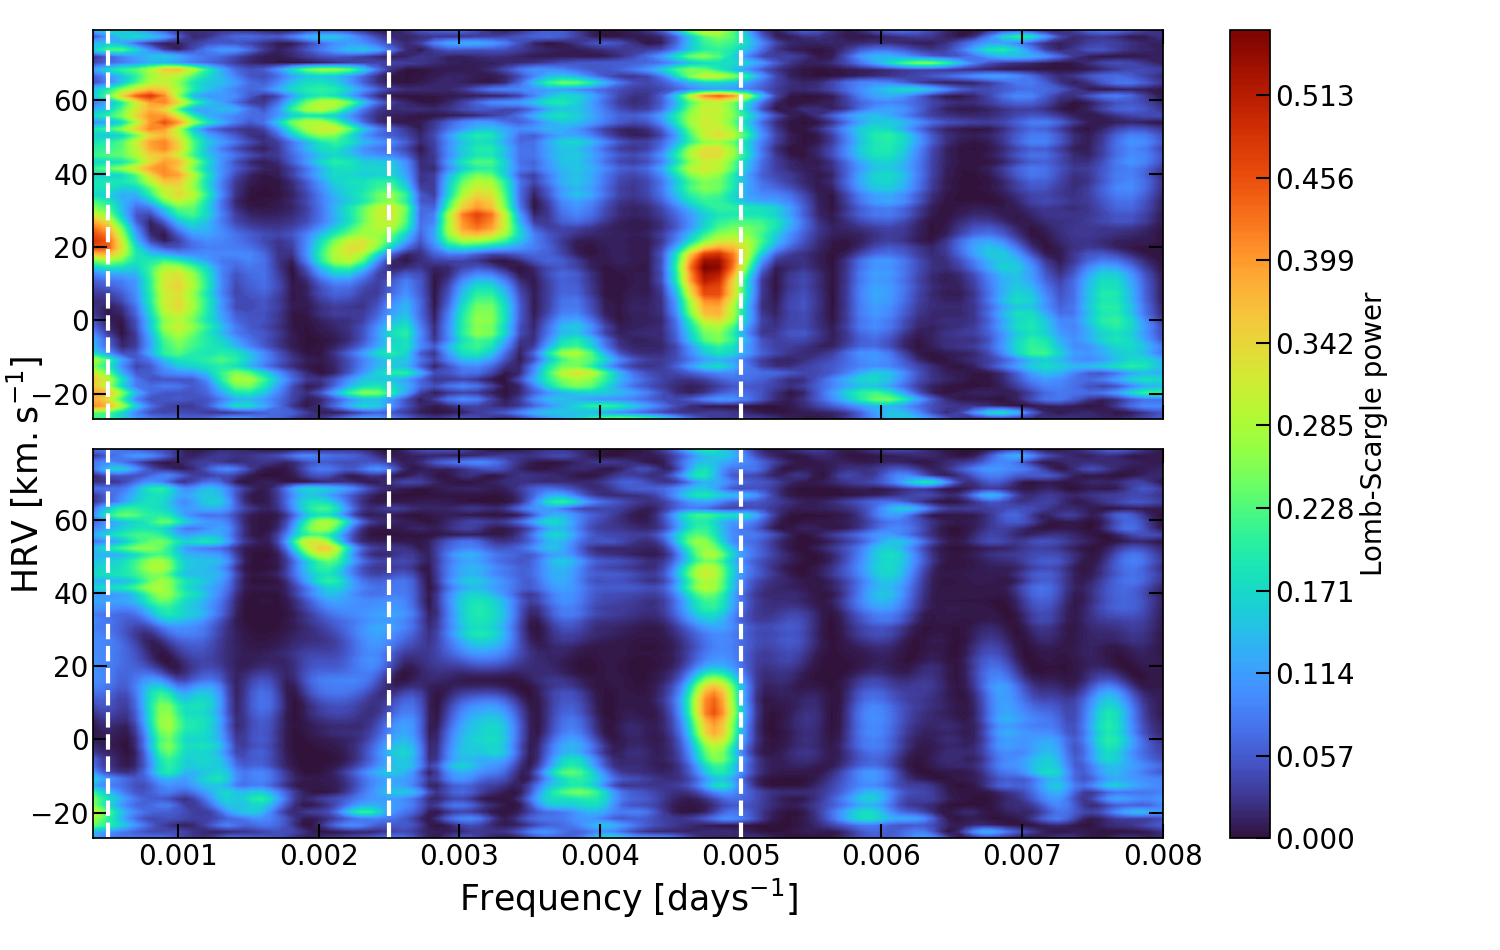
\includegraphics[width=0.5\textwidth]{Lomb-Scargle Stokes Q.png}
    \caption{Same as figure \ref{LS intensity} for stokes Q. }
    \label{LS Q}
\end{figure}

\begin{figure}[!h]
    \centering
    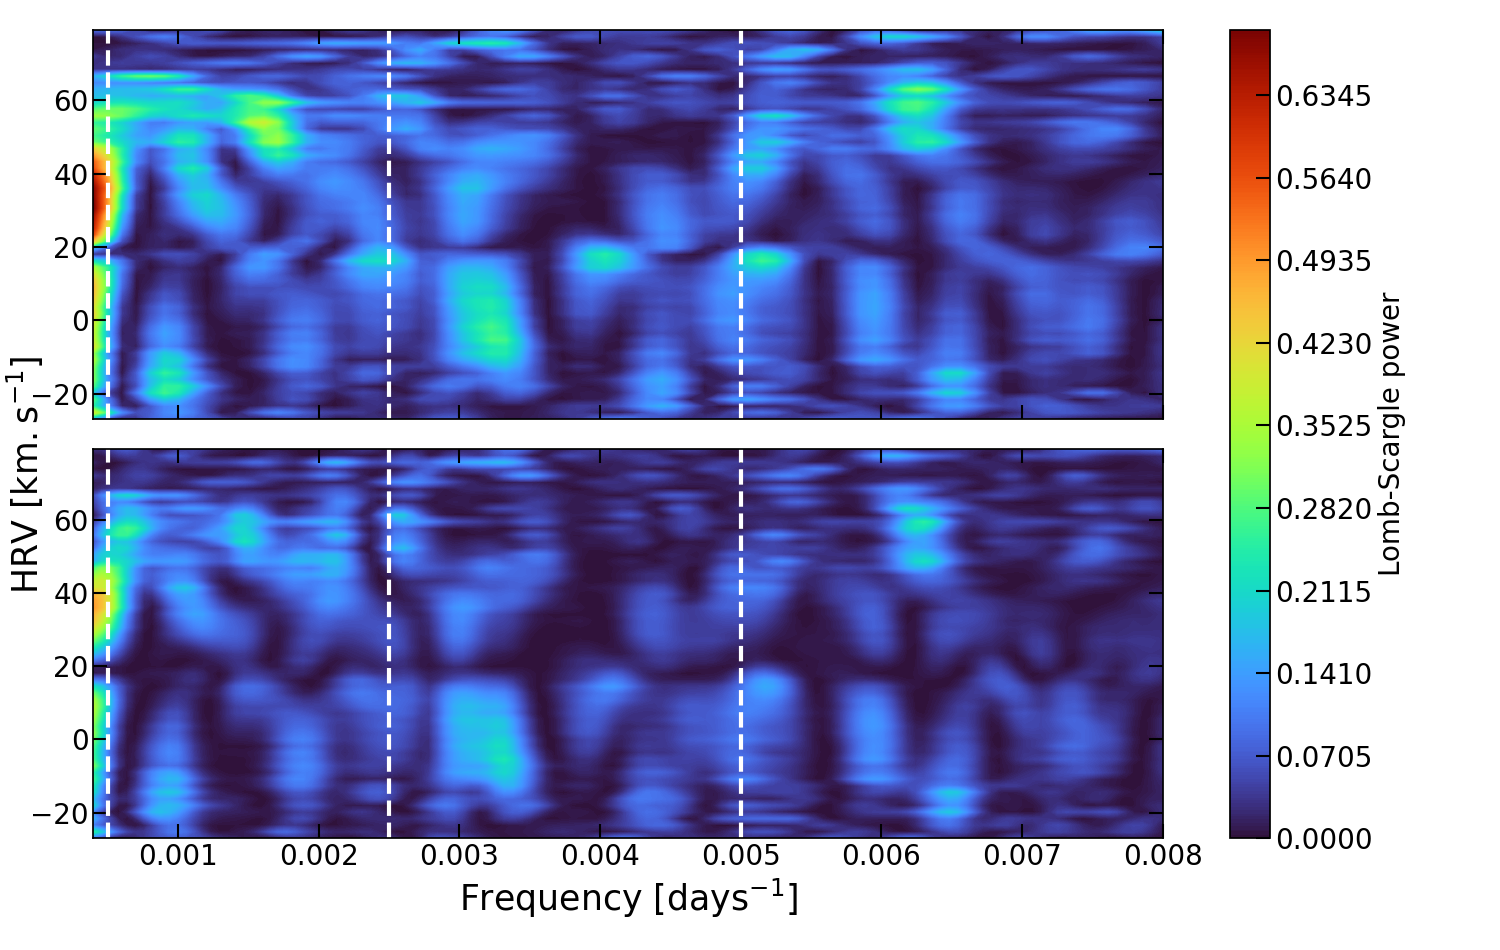
\includegraphics[width=0.5\textwidth]{Lomb-Scargle Stokes U.png}
    \caption{Same as figure \ref{LS intensity} for stokes U.}
    \label{LS U}
\end{figure}


\begin{figure}[!h]
    \centering
    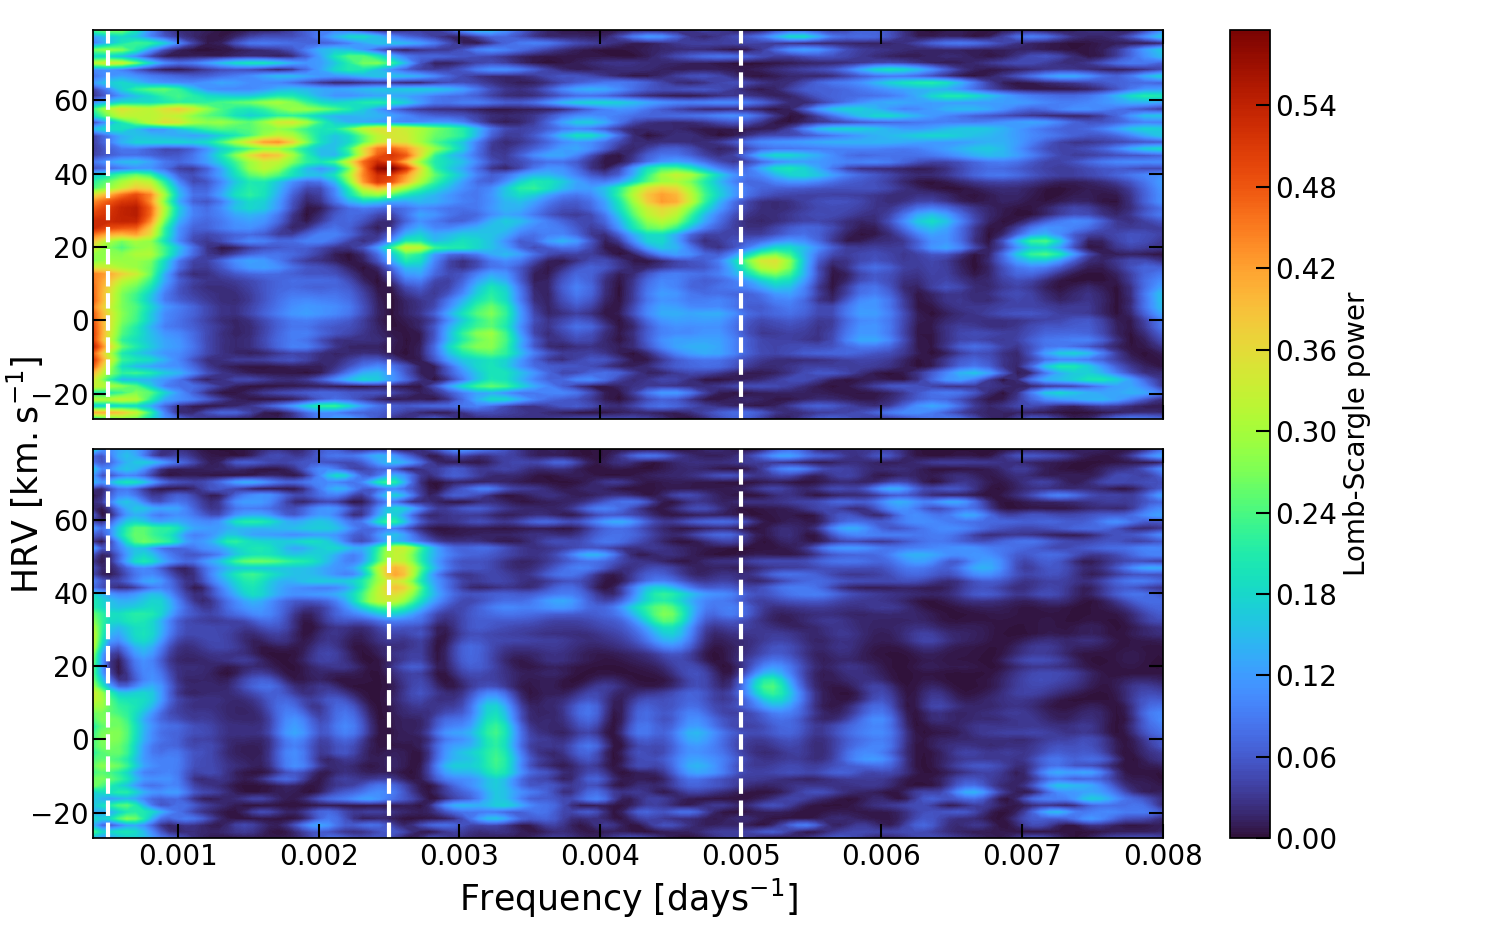
\includegraphics[width=0.5\textwidth]{Lomb-Scargle linear polarization.png}
    \caption{Same as figure \ref{LS intensity} for the linear polarization: $\sqrt{\mathrm{Q^2}+\mathrm{U^2}}$.}
    \label{LS linear polarization}
\end{figure}



%\section{Recovering the variability of Betelgeuse in the LSD profile}

%\subsection{Intensity}
Figure \ref{LS intensity} shows the LS periodogram of the LSD of the intensity profile. Interestingly, we recover the LSP at 2000 days, 
but located at a HRV of $\sim$ 20 km/s rather than over the whole profile. This periodicity is still present after the  dimming, but  it is located at a HRV between 0 and 10 km/s. 
There is also a weaker signal at the fundamental mode, around 400 days before the dimming. But this signal completely disappears after the dimming. From these observations
we find  hard to attribute 
the observed LS power to a global period of Betelgeuse.
%, however it might be a hint that this periodicity has changed after the dimming. 
Our results 
in the intensity profile are consistent with the one from \cite{mathias_evolution_2018} who used 2D fourier analysis and found that the dominant period was the LSP. 


\subsection{Stokes Q and U}

Figure \ref{LS Q} and \ref{LS U} show the LS periodogram of both stokes Q and U. It is clear that the LS periodogram is completely different 
from the intensity one. A strong signal is present in fig. \ref{LS Q} around 200 days. Once again, this signal is weaker after the dimming.
Concerning stokes U in fig. \ref{LS U}, it appears that we only recover the LSP, which once again, is weaker after the great dimming. 
Those periodograms rise a lot of questions: why is the 200 days period only present in stokes Q? Why not in stokes U or intensity? 
We will discuss about those questions in the next section. It also appears that stokes Q is not sensitive to the LSP, or to be more precise, 
it is much more sensitive to the 200 days period. From this, we can conclude that stokes Q evolves on a time scale much more closer to the first overtone 
mode than the LSP or even the fundamental mode. Since Stokes Q is sensitive  to different periods, we must conclude that it is due to other mechanisms
than the one behind the periodicitys observed in intensity. Linear polarization in Betelgeuse is interpreted to be a proxy of  convective cells,
so we can speculate that the signal present in the periodogram 
may be related to  the lifetime of convective cells. Such hypothesis is comforted by what we see in the 
LSD profiles of  Betelgeuse  whose shape is overhauled  in typical time scales of  a few months,  
Such time scales observed in the Stokes profiles and attributed to the convective time scales 
appear to explain the strong signal present at 200 days in the LS periodogram of Stokes Q. 


\subsection{The linear polarization}

Figure \ref{LS linear polarization} shows the LS periodogram of the total linear polarization of Betelgeuse: $\sqrt{\mathrm{Q^2+U^2}}$. 
Interestingly, the LS periodogram shows a strong power at 400 days and 2000 days. This signal is much more weaker after the dimming.
While the LSP is already present in the LS of intensity, here we recover the 400 days periodicity, often invoked in the literature. 
Nonetheless, the power of this period peaks at a HRV of around 40 km/s. We recall that this velocity is the rest velocity of the star. 
Every signal beyond this velocity is either due to  plasma sinking in Betelgeuse, or to plumes of plasma rising beyond and above the limb of the star. 
Such plumes from the back hemisphere haven been often seen in other red supergiants like $\mu$ Cep \citep{lopez_ariste_height_2023}. 
This suggests that both signals at these period of 400 days found in intensity and total linear polarisation 
could well be due to the periodic appearance of plumes in the back himisphere rising high enough to appear above
the visible limb and generating a supplementary source of brightness. Once again we find a plausible explanation 
of these periods unrelated to pulsations, but rather to the convective dynamics of the star.

% Up to this point, we want to pinpoint the two elements that are a clue 
% to understand the variability of Betelgeuse: the 400 days period is present in the linear polarization signal and also at a HRV above 40 km/s.
% In any case, from the linear polarization and the intensity profile, we recover the different periods of Betelgeuse. Since linear polarization is 
% associated to convection and because we recover the periods of Betelgeuse, the main mechanism behind the variability of Betelgeuse points toward surface convection.

\subsection{The variability of Betelgeuse inferred from polarimetry imaging}

Using linear polarization, \cite{lopez_ariste_convective_2018} have been able to reconstruct images of Betelgeuse that have been sucessfully compared 
to inteferometric images of \cite{montarges_close_2016}. The images are produced by finding the brightness distribution that better fits the observed linear 
polarization LSD profile using a Marquardt-Levemberg minimisation.

Betelgeuse is observed in average every other weeks by the TBL, and hence
we are able to follow its surface activity through polarimetry imaging. This has  allowed in the past the estimatation of  the size and the
 life time of the convective cells
at the surface. From these images, we can compute a photo-center, which is sensitive to the size and the number of convective cells. 
An homogeneous star will have a photo-center coinciding with barycenter of the star, whereas a star with one or two huge convective cells will have a
photo-center displacement more important, up to a few percent of the stellar radius in the case of RSG \citep{chiavassa_probing_2022}. 

Since the photo-center is linked to surface convection, it is worth checking for periods in its 
dynamics over the 13 years of observations of Betelgeuse at the TBL. Such periods will not 
be completely unrelated to the ones presented in the previous section, but will capture 
other aspects of the phenomena at work.

We computed the LS periodogram of the displacement of the photo-center. But, before going any further, we have to warn
 about the interpretation of such images. 
Linear polarization suffers from a $180 ^\circ$ degree ambiguity already mentioned in \cite{auriere_discovery_2016}. For that reason, our images 
can be 
rotated by $180^\circ$ degree, and the brightness distribution will still fit the observed LSD polarization profiles. 
If a particular observation were to be treated independently of previous observations, the solution found by 
the algorithm could be any of the ambigous solutions possible. To obtain a continuity 
between the series images, 
for a given day we use the brightness distribution of the previous day as initial point 
of the  fitting iteration; and for the first image, we start with a 
random brightness distribution as the beginning of the fit. 
Even though we are able to produce a series of images  consistent with each other, it is important 
to keep in mind that the photo-center displacement computed from the series 
will be affected by the choice of the first image. 
To overcome this issue, we decided to compute
the photo-center displacement from 100 different initial parameters and their subsequent series 
of images in an effort to recover from the ensemble
properties that are independent of the choice of the first image. 

\begin{figure}[!h]
    \centering
    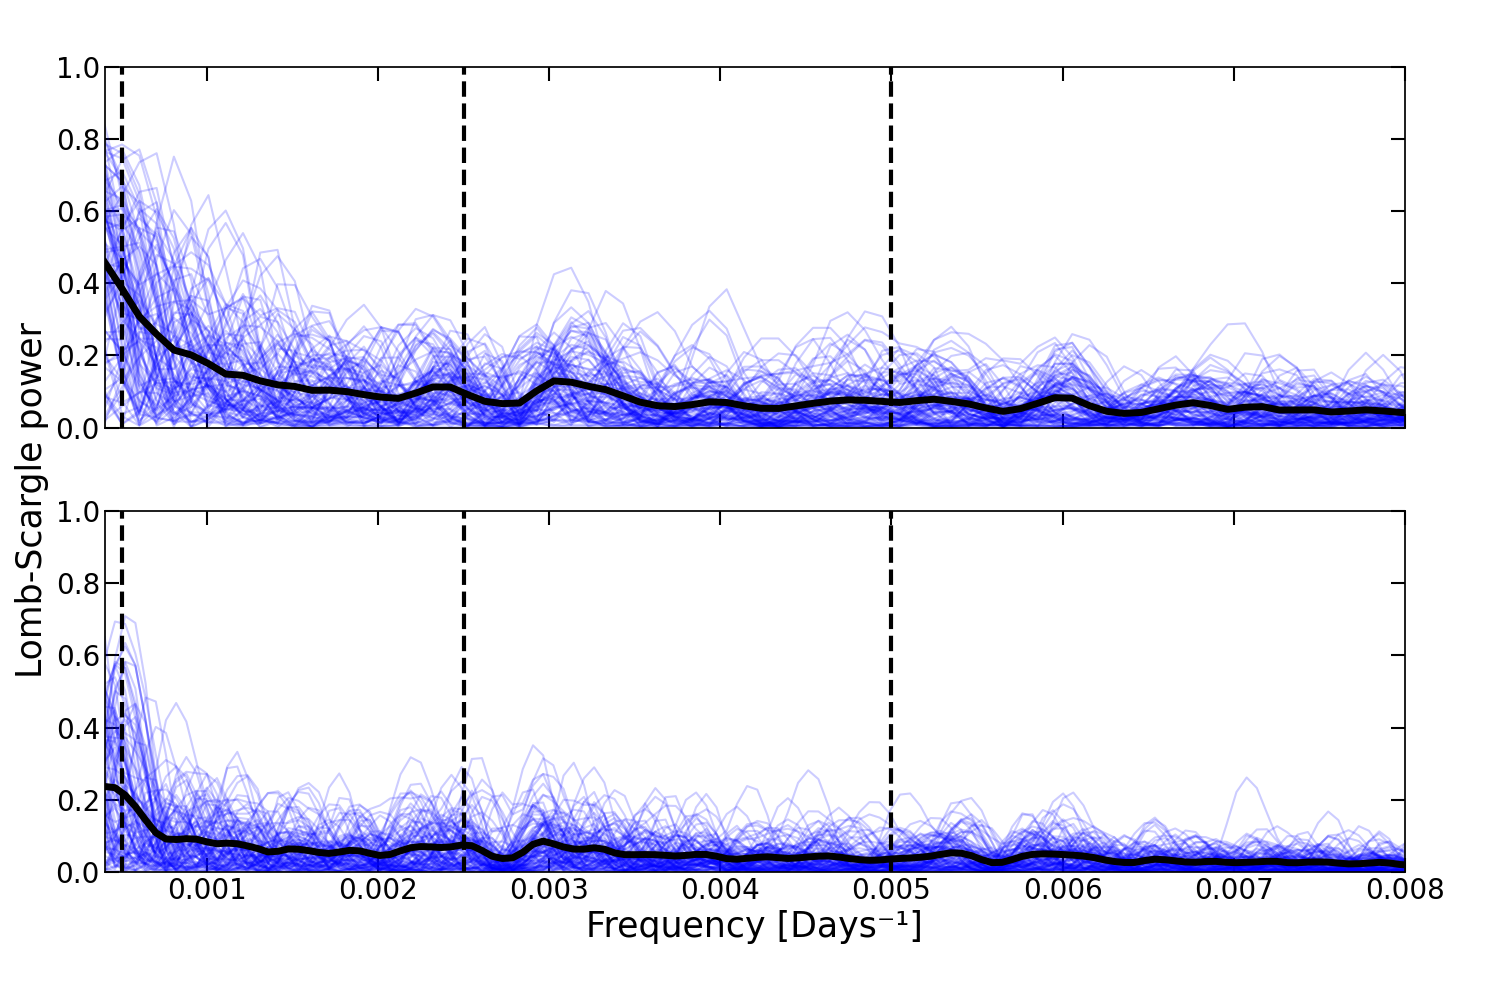
\includegraphics[width=0.5\textwidth]{Lomb-Scargle Photo-center.png}
    \caption{Lomb-Scargle periodogram of the 100 photo-center displacement of Betelgeuse. Each blue curve corresponds to a LS periodogram of one photo-center
     displacement. The black line is the average of the 100 LS periodogram. The black dashed lines represent the 2000, 400 and 200 days period respectively 
     (from left to right). The upper panel is the LS from data before the dimming. The lower panel is the LS from the all dataset, 
     including data after the great dimming. }
    \label{LS photocenter}
\end{figure}

Figure \ref{LS photocenter} shows the LS periodogram of the photo-center displacement  of each one of those 100 series (blue lines) and the average LS periodogram (black line). 
As before, the upper panel shows the LS from images before the great dimming of Betelgeuse only, whereas the lower panel is the LS for the whole set of 
data,  including images after the dimming. The black dashed lines mark the 2000, 400 and 
200 days periods respectively. First, we find the the LS power is high around the LSP, though
uncomfortably close to the auto-correlation peak.
We also notice a decrease in the Lomb-Scargle power from  before to after the dimming, in 
concurrence to what was seen in the LS periodograms of the LSD profiles. Before it, there are two smalls bumps around the 400 days period. 
But those bumps almost completely disappear after the dimming. Even though it is 
hard to identify the 400 days period from those bumps alone,
we still find that there is a difference before and after the dimming. 
And this is concluded  from images that exclusively involve surface convection.
The LS of the photo-center displacement points towards a variability explained by convection only. 
And this is consistent with what we obtained from linear polarization.
%Both the photo-center displacement and the LS of the linear polarization point toward a variability explained by surface convection.  

\subsection{The variability of the light curve of Betelgeuse}

After examining the periods found by the Lomb-Scargle technique on the polarization data, and its derivatives, obtained by the TBL over the last 
13 years, it is worth putting them in the context of the periods found traditionally on light curves over the same period of time. Two aspects 
are of our interest in this comparison: the behaviour of the light curve before and after the great dimming, and the amplitudes of the peaks 
at the main cited periods.

% In the literature, it is reported that before the great dimming the main period of Betelgeuse was of 400 days \citep{kiss_variability_2006}. 
% This pulsation is often associated to the fundamental pressure mode. After the dimming, however this period appears to have disappeared 
% and only the period at 200 days,  associated to the first overtone of the fundamental mode, is visible since. 
% No explanations based upon pulsations have been ofered concerning this change of variability after or perhaps because of the dimming. But this 
% is a behaviour that

We have recovered the light curve of Betelgeuse in the visible from the AAVSO database for the last 13 years (Figure \ref{light curve Betelgeuse}).
Before the great dimming, the magnitude of Betelgeuse evolves on a timescale of a year, whereas after the dimming, the variability of Betelgeuse has changed. 
It is clear from fig. \ref{light curve Betelgeuse} that the 
variability of Betelgeuse is evolving on a timescale shorter than one year. This qualitative change has been pointed out before.
In the literature, it is reported that before the great dimming the main period of Betelgeuse was of 400 days \citep{kiss_variility_2006}. 
This period is often associated to the fundamental pressure mode. After the dimming, however this period appears to have disappeared 
and only the period at 200 days,  associated to the first overtone of the fundamental mode, is visible since \citep{XXX}.
No explanations based upon pulsations have been ofered concerning this change of variability after or perhaps because of the dimming. But this 
is a behaviour that fully concurs with what we find in the polarization data, and which cannot be related to any stellar pulsation but rather 
convective dynamics. Beyond the actual values of the periods found in a Lomb-Scargle periodogram, we also see a correspondence between polarization 
and the light curve in these changes in the observed periods before and after the great dimming. Such concurrence points to an explanation 
in terms of convective dynamics also for the variability of the light curve.


It may be argued that the periodograms presented in the previous sections and, in particular, those  of the photo-center displacements, 
present low amplitude peaks at the referred main periods. One may wonder whether we are over-interpreting mere fluctuations of the periodograms, 
while the peaks seen in the literature from analysis of the light curve are unmistakable. It is therefore worth to take advantage of the 
availability of the AAVSO data to perform a Lomb-Scargle periodogram of the light curve in the same period covered by our polarization data and,
furthermore, taking into consideration data around the dates for which TBL data is available. Periodograms  with such constraints are 
shown in Fig.\ref{LSAAVSO}. Even when the full dataset for the period is taken into account, the periods present small amplitudes, and are 
fully and favourably comparable with the periodograms presented above. This is even more dramatic when the periodogram is made from data at the exclusive 
dates at which TBL data is available. It stands out that the low amplitude peaks are rather due to both the sparse cadence and short span of 
time of the TBL data series rather than to a physical absence. Actually, the present tests puts more emphasis on the importance of the 
strong peaks seen at selected wavelengths in the LSD profiles, strong when compared to the peaks at similar periods arising from the light curve. 





% constant, which is not consistent with a pulsating scenario. The constant magnitude of Betelgeuse points toward another scenario than pulsation. Using surface 
% convection, we can fully explain the variability of Betelgeuse. The oscillations in the light curve are due to two mechanisms: surface convection and rising 
% plumes of plasma beyond the limb of the star. This last mechanism being random, it happens from time to time. The timescale on which convective cells evolve
% is between one and two years, which is also consistent with the 400 days period found in the literature.  After the dimming, the change of periodicity in the
% light curve is explained by surface convection, the random variation of brightness distribution could lead to the 200 days periodicity found in the literature. 
% The constant brightness of Betelgeuse for the last 6 months is explainable by the same random brightness distribution: the surface of Betelgeuse is calm, 
% leading to this constant brightness. In the future, we expect to see the light curve of Betelgeuse to change, maybe with another main period, but which 
% is in fact caused by surface convection. Thus, the main mechanism in the variability of Betelgeuse is surface convection, which is sufficient to explain the 
% variation in the magnitude of Betelgeuse.  


\begin{figure}[!h]
    \centering
    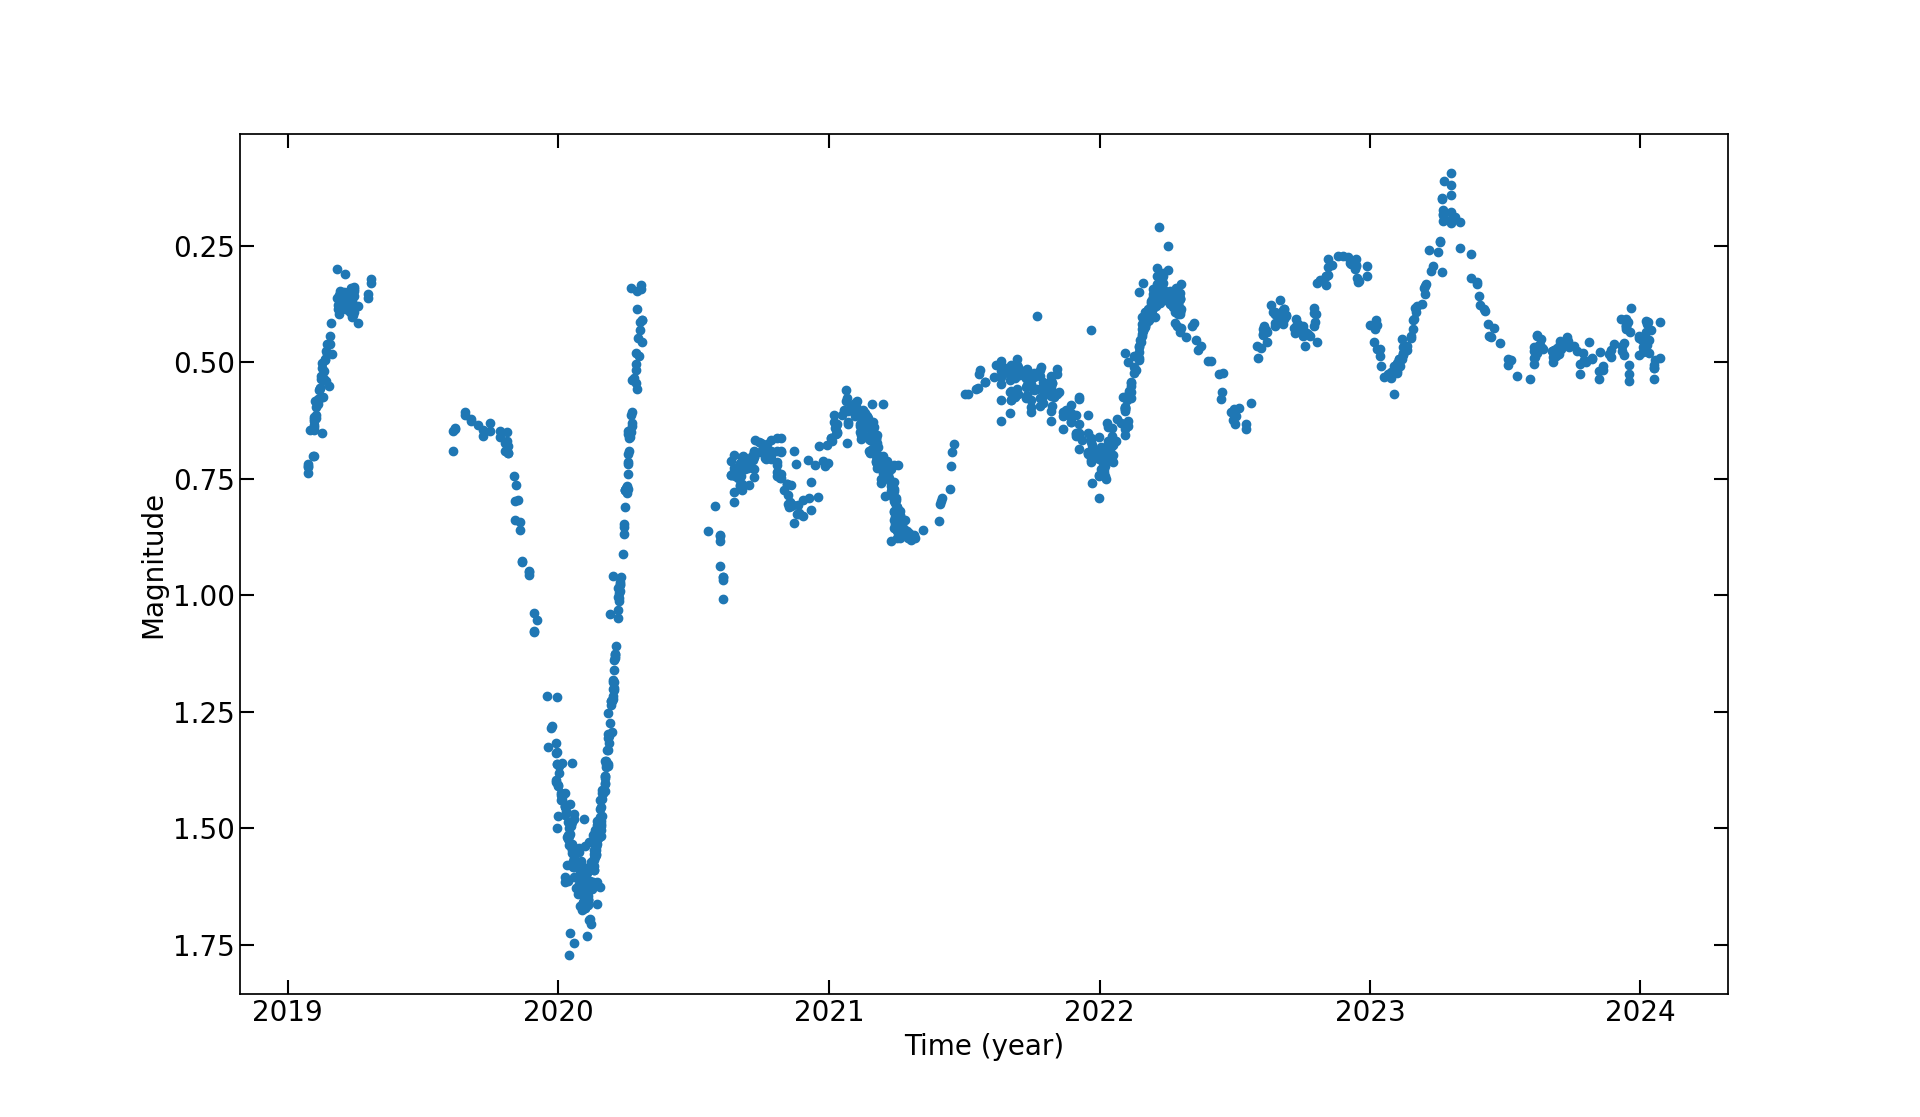
\includegraphics[width=0.5\textwidth]{Light_curve_Betelgeuse.png}
    \caption{Light curve of Betelgeuse from AAVSO in the V-band.}
    \label{light curve Betelgeuse}
\end{figure}


\section{Surface convection suffices to explain the observed variability}

Before summing up the conclusions of this work, we can afford proposing alternative scenarios for the observed periodicities in the light curve, 
the LSD profiles and the displacement of the photo-center of the inferred photospheric image reconstructions. The presence of the same 
periods and, after taking into consideration the time span and sparsity of the TBL data series, the larger amplitude of the peaks in
polarization data  than in the light curve point to a common origin, one that is rather based upon convective dynamics and not to radial or 
other global pulsations.

% We recall that while the nature of the LSP is still in debate, the nature of the lower periods is quite commonly 
% attributed to  pressure modes 
% (e.g \cite{kiss_variability_2006}). The mechanism behind the pulsation of Betelgeuse is attributed to the $\kappa$-mechanism. In this 
% section, we attempt to 
% find an explanation to the 400 days periodicity of Betelgeuse. 
% As mentioned before, the LS periodogram of linear polarization shows a periodicity 
% around 400 days. Furthermore, the region where the LS power is high is around 40km/s. 
% This wavelength corresponds to most redshifted signal present in Betelgeuse.

The 400-day period appears prominently in both the intensity and the total polarization profiles. And in both cases, it is mostly present 
at wavelengths in the red wing, often beyond the 40 km/s value.
We recall that in the present scenario for the formation of the polarization signal, this signal is supposed to remain between 
-20 and 40km/s. Signals above 40km/s are uncommon and can be associated to
 plasma rising behind the limb of Betelgeuse. 
Such scenario has been observed in the RSG $\mu$ Cep and was introduced by \cite{lopez_ariste_height_2023} to explain the excess of 
linear polarization beyond  the rest velocity of the star, which for Betelgeuse is fixed at +40km/s. 
In $\mu$ Cep, such  linear polarization signal beyond the limit of the rest velocity of the star is very strong and particularly 
common, two features that prompted a dedicated explanation. In Betelgeuse, such signals, when present, are weaker. However, 
they are visible from time to time, with regularities that are captured by  the LS periodogram at 400 days.
Without further justification, we may propose that convective plumes in the hidden hemisphere of the star and 
rising above the limb from time to time are responsible for the  400 days period in the light curve. When such plumes rise high enough 
to be geometrically visible above the limb they show signals in intensity and polarization at redshifted wavelengths. They also
 increase the emitting surface of the star and  the number of photons that we receive,
leading to an increase of the brightness visible in the light curve. After a few weeks or months, the plume falls back to Betelgeuse, 
disappearing from our point of view,  leading to a decrease of the brightness.

The appearance of such high-rising plumes is not necessarily periodic. And the star can easily shift from active periods when such 
plumes are a common feature to calmer periods when no plume is visible for months. $\mu$ Cep may be in one such active period presently,
while Betelgeuse may have experienced recently one great such event in the direction of the Earth that, after dust formed, became the great 
dimming, but since then no other high-rising plume has appeared, explaining the absence of the 400-day period since the great dimming. 
From the point of view of convective dynamics we can offer an explanation of the 400-day period which not only explains the observation of 
this period both in the light curve and in the polarization profiles, but also its presence at redshifted wavelengths and its present (and probably 
temporary) disappearance since the great dimming.


% This is exactly what we see in the LSD profile of the linear polarization of Betelgeuse: 
% from time to time, there is a net signal above 40km/s, which is present for a few weeks, and then disappears. Since this signal is not always present, 
% it is found by the LS periodogram as a periodic event. However, it is not periodic at all: because the plumes rise at random moments, sometimes they 
% appear every years, sometime they do not. This would explain why we only see it before the dimming. After the dimming, this kind of event never happened 
% for the moment. Thus, the LS periodogram, at that precise frequency, finds that there is a periodic signal before the dimming, but not after, leading to
% a lower LS power at this frequency.

Concerning the 200 days period, we notice that it coincides with  the typical timescales on which the Stokes parameters evolve. 
The 
LSD profiles of stokes Q or U will slightly change when we observe Betelgeuse every two weeks. But they are completely overhauled 
on time scales of several months. The Lomb-Scargle perioograms appear to capture this spectral dynamic around periods of 200 days.
 Such changes in the profiles are directly linked to the dynamics of the surface,  to  the evolution and movements 
of convective cells over the visible hemisphere. So the 200-day period appears to be related to the evolution of the convective patterns 
on the surface of Betelgeuse. 
 As showed by
\cite{lopez_ariste_convective_2018}, some of those convective cells can live up for years. We may speculate
that the LSP may be related to those long living structures. However the present span of data from the TBL is insufficient to do more than
just speculate. It should be noticed that  
 the peak is not present in stokes U, and this may point to a more stochastic event than just long-living structures.

% To summarise what we have done so far: we were able to explain the variability of Betelgeuse using surface convection only. The convective cells play 
% the most important role in the variability of Betelgeuse. Our work does not need pulsation to explain its variability. This does not mean that there are 
% no pulsation in Betelgeuse. What we claim is that the most important factor in the variability of Betelgeuse is the timescale on which the convective 
% cells evolve. Pulsation could exist on Betelgeuse, but they are not the main contributor to the variability. 




\section{Conclusion}

The main observation  presented in this work is that the very same periods identified in the light curve of Betelgeuse are also seen in the intensity and polarization
spectra measured with the TBL. Periods in the light curve have often been traditionally associated to pulsation due to pressure modes. But 
such pulsation would in no case affect the polarisation signals nor would explain the fact that the periods can be observed with stronger 
amplitude at selected wavelengths but no others.  Pulsation appears to offer no coherent explanation to these observations, are hardly to the 
observed changes in the variability since the great dimming.  The concurrence of observational facts, actual period values, evolution before 
and after the dimming, the larger amplitude of the period peaks in polarizarion data, points towards a common origin for those variabilities. 
And such origin cannot be pulsations.

The interpretaion of the linear polarization profiles is made in terms of convective structures in the atmosphere of Betelgeuse. We suggest 
that it is in these convective structures and their temporal evolution that we will find the true reason for the observed periodicities both 
in the light curve and in the spectropolarimetric observations. This is the main conclusion of this work: the observed periods are related 
to convective dynamics and not to radial pulsations of the star.

Although of secondary importance, we may suggest with more or less ease what phenomena are at the origin of the main periods. The 400-day period 
appears to be strongly related to the appearence of plumes in the back hemisphere of the star rising high enough to be seen above the limb.
Such plumes have been described in another RSG, $\mu$ Cep, and while less common or prominent, they are also present in Betelgeuse. The irregularity 
of their presence justifies the 400-day period, which is captured by the Lomb-Scargle periodogram in the polarization signals attributed to 
this phenomenon. The redshifted wavelengths at which this periodicity is found are justified by the plume moving away of the star and of the Earth while 
raising in the back hemisphere, while the brightness increase is justified by the extra surface of emitting plasma visible. The 200-day period is less 
prominent but appears to be correlated to the typical time scales of the evolution of the convective structures themselves on the visible hemisphere. 
The LSP origin is harder to pinpoint given the insufficient time length of our time series. One can speculate if it may be related to the 
longest living photospheric structures, but this explanation does not adequately explain all the features associated to this period. Longer time 
series of spectropolarimetric observations of Betelgeuse will be required to shed light on this.




\begin{acknowledgements}
    This work was supported by the "Programme National de Physique Stellaire" (PNPS) of CNRS/INSU co-funded by CEA and CNES.
    We acknowledge support from the French National Research Agency (ANR)
    funded project PEPPER (ANR-20-CE31-0002)
    An acknowledgement to the AAVSO may be required??????????????????
    \end{acknowledgements}
    
    \bibliographystyle{aa}
    %\bibliographystyle{aa}
    
    \bibliography{art75}
\end{document}